%%%%%%%%%%%%%%%%%%%%%%%%%%%%%%%%%%%%%%%%%
% Classicthesis Typographic Thesis
% LaTeX Template
% Version 1.0 (23/4/12)
%
% This template has been downloaded from:
% http://www.LaTeXTemplates.com
%
% Original author:
% Andr� Miede (http://www.miede.de)
%
% License:
% CC BY-NC-SA 3.0 (http://creativecommons.org/licenses/by-nc-sa/3.0/)
%
% General Tips:
% 1) Make sure to edit the classicthesis-config.file
% 2) New enumeration (A., B., C., etc in small caps): \begin{aenumerate} \end{aenumerate}
% 3) For margin notes: \marginpar or \graffito{}
% 4) Do not use bold fonts in this style, it is designed around them
% 5) Use tables as in the examples
% 6) See classicthesis-preamble.sty for useful commands
%
%%%%%%%%%%%%%%%%%%%%%%%%%%%%%%%%%%%%%%%%%

%----------------------------------------------------------------------------------------
%	PACKAGES AND OTHER DOCUMENT CONFIGURATIONS
%----------------------------------------------------------------------------------------

\documentclass[
		twoside,openright,titlepage,numbers=noenddot,headinclude,%1headlines,
                footinclude=true,cleardoublepage=empty,
                BCOR=5mm,paper=a4,fontsize=11pt, % Binding correction, paper type and font size
                ngerman,american, % Languages
                ]{scrreprt} 
                
% Includes the file which contains all the document configurations and packages - make sure to edit this file
%%%%%%%%%%%%%%%%%%%%%%%%%%%%%%%%%%%%%%%%%
% Thesis Configuration File
%
% The main lines to change in this file are in the DOCUMENT VARIABLES
% section, the rest of the file is for advanced configuration.
%
%%%%%%%%%%%%%%%%%%%%%%%%%%%%%%%%%%%%%%%%%

%----------------------------------------------------------------------------------------
%	DOCUMENT VARIABLES
%	Fill in the lines below to enter your information into the thesis template
%	Each of the commands can be cited anywhere in the thesis
%----------------------------------------------------------------------------------------

% Remove drafting to get rid of the '[ Date - classicthesis version 4.0 ]' text at the bottom of every page
\PassOptionsToPackage{eulerchapternumbers,listings,drafting, pdfspacing, subfig,beramono,eulermath,parts,dottedtoc}{classicthesis}
% Available options: drafting parts nochapters linedheaders eulerchapternumbers beramono eulermath pdfspacing minionprospacing tocaligned dottedtoc manychapters listings floatperchapter subfig
% Adding 'dottedtoc' will make page numbers in the table of contents flushed right with dots leading to them

\newcommand{\myTitle}{GIRAF Launcher\xspace}
\newcommand{\mySubtitle}{An Homage to The Elements of Typographic Style\xspace}
\newcommand{\myDegree}{Doktor-Ingenieur (Dr.-Ing.)\xspace}
\newcommand{\myName}{Andr\'e Miede\xspace}
\newcommand{\myProf}{Put name here\xspace}
\newcommand{\myOtherProf}{Put name here\xspace}
\newcommand{\mySupervisor}{Put name here\xspace}
\newcommand{\myFaculty}{Put data here\xspace}
\newcommand{\myDepartment}{Put data here\xspace}
\newcommand{\myUni}{Put data here\xspace}
\newcommand{\myLocation}{Darmstadt\xspace}
\newcommand{\myTime}{December 2011\xspace}
\newcommand{\myVersion}{version 4.0\xspace}

%----------------------------------------------------------------------------------------
%	USEFUL COMMANDS
%----------------------------------------------------------------------------------------

\newcommand{\ie}{i.\,e.}
\newcommand{\Ie}{I.\,e.}
\newcommand{\eg}{e.\,g.}
\newcommand{\Eg}{E.\,g.} 

\newcounter{dummy} % Necessary for correct hyperlinks (to index, bib, etc.)
\providecommand{\mLyX}{L\kern-.1667em\lower.25em\hbox{Y}\kern-.125emX\@}

%----------------------------------------------------------------------------------------
%	PACKAGES
%----------------------------------------------------------------------------------------

\usepackage{lipsum} % Used for inserting dummy 'Lorem ipsum' text into the template

%------------------------------------------------
 
\PassOptionsToPackage{latin9}{inputenc} % latin9 (ISO-8859-9) = latin1+"Euro sign"
\usepackage{inputenc}
 
 %------------------------------------------------

%\PassOptionsToPackage{ngerman,american}{babel}  % Change this to your language(s)
% Spanish languages need extra options in order to work with this template
%\PassOptionsToPackage{spanish,es-lcroman}{babel}
\usepackage{babel}

%------------------------------------------------			

\PassOptionsToPackage{square,numbers}{natbib}
 \usepackage{natbib}
 
 %------------------------------------------------

\PassOptionsToPackage{fleqn}{amsmath} % Math environments and more by the AMS 
 \usepackage{amsmath}
 
 %------------------------------------------------

\PassOptionsToPackage{T1}{fontenc} % T2A for cyrillics
\usepackage{fontenc}

%------------------------------------------------

\usepackage{xspace} % To get the spacing after macros right

%------------------------------------------------

\usepackage{mparhack} % To get marginpar right

%------------------------------------------------

\usepackage{fixltx2e} % Fixes some LaTeX stuff 

%------------------------------------------------

\PassOptionsToPackage{smaller}{acronym} % Include printonlyused in the first bracket to only show acronyms used in the text
\usepackage{acronym} % nice macros for handling all acronyms in the thesis

%------------------------------------------------

%\renewcommand*{\acsfont}[1]{\textssc{#1}} % For MinionPro
\renewcommand{\bflabel}[1]{{#1}\hfill} % Fix the list of acronyms

%------------------------------------------------

\PassOptionsToPackage{pdftex}{graphicx}
\usepackage{graphicx} 

%----------------------------------------------------------------------------------------
%	FLOATS: TABLES, FIGURES AND CAPTIONS SETUP
%----------------------------------------------------------------------------------------

\usepackage{tabularx} % Better tables
\setlength{\extrarowheight}{3pt} % Increase table row height
\newcommand{\tableheadline}[1]{\multicolumn{1}{c}{\spacedlowsmallcaps{#1}}}
\newcommand{\myfloatalign}{\centering} % To be used with each float for alignment
\usepackage{caption}
\captionsetup{format=hang,font=small}
\usepackage{subfig}  

%----------------------------------------------------------------------------------------
%	CODE LISTINGS SETUP
%----------------------------------------------------------------------------------------

\usepackage{listings} 
\usepackage{color} %For sourceCode listnings

%\lstset{emph={trueIndex,root},emphstyle=\color{BlueViolet}}%\underbar} % for special keywords
\lstset{language=[LaTeX]Tex, % Specify the language for listings here
keywordstyle=\color{RoyalBlue}, % Add \bfseries for bold
basicstyle=\small\ttfamily, % Makes listings a smaller font size and a different font
%identifierstyle=\color{NavyBlue}, % Color of text inside brackets
commentstyle=\color{Green}\ttfamily, % Color of comments
stringstyle=\rmfamily, % Font type to use for strings
numbers=left, % Change left to none to remove line numbers
numberstyle=\scriptsize, % Font size of the line numbers
stepnumber=5, % Increment of line numbers
numbersep=8pt, % Distance of line numbers from code listing
showstringspaces=false, % Sets whether spaces in strings should appear underlined
breaklines=true, % Force the code to stay in the confines of the listing box
%frameround=ftff, % Uncomment for rounded frame
frame=single, % Frame border - none/leftline/topline/bottomline/lines/single/shadowbox/L
belowcaptionskip=.75\baselineskip % Space after the "Listing #: Desciption" text and the listing box
}


%%%%%%%%%%%%%%%%%%%%%%%%
%% Steiniche was here %%
%%%%%%%%%%%%%%%%%%%%%%%%
\definecolor{gray95}{gray}{.95}
\lstdefinestyle{sourceCode}
{ 
 numbers=left,
 numbersep=5pt, 
 stepnumber=1,
 captionpos=b,  %bottom
 keywordstyle=\color{purple},
 commentstyle=\color[rgb]{0.133,0.545,0.133},
 stringstyle=\color[rgb]{0.627,0.126,0.941},
 backgroundcolor=\color{gray95},
 frame=lrtb,
 framerule=0.5pt,
 linewidth=\textwidth,
 tabsize=4,
 numberbychapter=true,
 basicstyle=\ttfamily\footnotesize,
 language=[Sharp]C,
 breaklines=true,
 showstringspaces=false,
 emph=[2]{Tag,Problem,Person,List,NotSupportedException,TestMethod,ProblemSearch,Assert,
 EntityCollection,Department,IEnumerable,TimeSpan,DateTime},%%Classes
 emphstyle=[2]{\color[rgb]{0.1,0.5,0.5}},
 float=htb,
 breakindent=20pt
}



%----------------------------------------------------------------------------------------
%	Quoteations
%----------------------------------------------------------------------------------------
\newcolumntype{R}{>{\raggedleft\arraybackslash}X}%

\def\changemargin#1#2{\list{}{\rightmargin#2\leftmargin#1}\item[]}
\let\endchangemargin=\endlist
\newcommand{\myQuoteA}[2]{
\begin{changemargin}{.7in}{.7in}
\textbf{``}
#1
\textbf{''}
\ifthenelse{\isempty{#2}}%  If there is nothing stated here just print the shit. 
{}% if #1 true
{\vspace{-3mm}\begin{changemargin}{.9in}{.7in}\raggedleft{{\footnotesize--- #2}}\end{changemargin}}% if #1 false
\end{changemargin}
}

\newcommand{\myQuote}[1]{\myQuoteA{#1}{}}

%----------------------------------------------------------------------------------------
%	HYPERREFERENCES
%----------------------------------------------------------------------------------------

\PassOptionsToPackage{pdftex,hyperfootnotes=false,pdfpagelabels}{hyperref}
\usepackage{hyperref}  % backref linktocpage pagebackref
\pdfcompresslevel=9
\pdfadjustspacing=1

\hypersetup{
% Uncomment the line below to remove all links (to references, figures, tables, etc)
%draft, 
colorlinks=true, linktocpage=true, pdfstartpage=3, pdfstartview=FitV,
% Uncomment the line below if you want to have black links (e.g. for printing black and white)
%colorlinks=false, linktocpage=false, pdfborder={0 0 0}, pdfstartpage=3, pdfstartview=FitV, 
breaklinks=true, pdfpagemode=UseNone, pageanchor=true, pdfpagemode=UseOutlines,
plainpages=false, bookmarksnumbered, bookmarksopen=true, bookmarksopenlevel=1,
hypertexnames=true, pdfhighlight=/O, urlcolor=webbrown, linkcolor=RoyalBlue, citecolor=webgreen,
%------------------------------------------------
% PDF file meta-information
pdftitle={\myTitle},
pdfauthor={\textcopyright\ \myName, \myUni, \myFaculty},
pdfsubject={},
pdfkeywords={},
pdfcreator={pdfLaTeX},
pdfproducer={LaTeX with hyperref and classicthesis}
%------------------------------------------------
}   

%----------------------------------------------------------------------------------------
%	BACKREFERENCES
%----------------------------------------------------------------------------------------

\usepackage{ifthen} % Allows the user of the \ifthenelse command
\newboolean{enable-backrefs} % Variable to enable backrefs in the bibliography
\setboolean{enable-backrefs}{false} % Variable value: true or false

\newcommand{\backrefnotcitedstring}{\relax} % (Not cited.)
\newcommand{\backrefcitedsinglestring}[1]{(Cited on page~#1.)}
\newcommand{\backrefcitedmultistring}[1]{(Cited on pages~#1.)}
\ifthenelse{\boolean{enable-backrefs}} % If backrefs were enabled
{
\PassOptionsToPackage{hyperpageref}{backref}
\usepackage{backref} % to be loaded after hyperref package 
\renewcommand{\backreftwosep}{ and~} % separate 2 pages
\renewcommand{\backreflastsep}{, and~} % separate last of longer list
\renewcommand*{\backref}[1]{}  % disable standard
\renewcommand*{\backrefalt}[4]{% detailed backref
\ifcase #1 
\backrefnotcitedstring
\or
\backrefcitedsinglestring{#2}
\else
\backrefcitedmultistring{#2}
\fi}
}{\relax} 

%----------------------------------------------------------------------------------------
%	AUTOREFERENCES SETUP
%	Redefines how references in text are prefaced for different 
%	languages (e.g. "Section 1.2" or "section 1.2")
%----------------------------------------------------------------------------------------

\makeatletter
\@ifpackageloaded{babel}
{
\addto\extrasamerican{
\renewcommand*{\figureautorefname}{Figure}
\renewcommand*{\tableautorefname}{Table}
\renewcommand*{\partautorefname}{Part}
\renewcommand*{\chapterautorefname}{Chapter}
\renewcommand*{\sectionautorefname}{Section}
\renewcommand*{\subsectionautorefname}{Section}
\renewcommand*{\subsubsectionautorefname}{Section}
}
\addto\extrasngerman{
\renewcommand*{\paragraphautorefname}{Absatz}
\renewcommand*{\subparagraphautorefname}{Unterabsatz}
\renewcommand*{\footnoteautorefname}{Fu\"snote}
\renewcommand*{\FancyVerbLineautorefname}{Zeile}
\renewcommand*{\theoremautorefname}{Theorem}
\renewcommand*{\appendixautorefname}{Anhang}
\renewcommand*{\equationautorefname}{Gleichung}
\renewcommand*{\itemautorefname}{Punkt}
}
\providecommand{\subfigureautorefname}{\figureautorefname} % Fix to getting autorefs for subfigures right
}{\relax}
\makeatother

%----------------------------------------------------------------------------------------

\usepackage{classicthesis} 

%----------------------------------------------------------------------------------------
%	CHANGING TEXT AREA 
%----------------------------------------------------------------------------------------

%\linespread{1.05} % a bit more for Palatino
%\areaset[current]{312pt}{761pt} % 686 (factor 2.2) + 33 head + 42 head \the\footskip
%\setlength{\marginparwidth}{7em}%
%\setlength{\marginparsep}{2em}%

%----------------------------------------------------------------------------------------
%	USING DIFFERENT FONTS
%----------------------------------------------------------------------------------------

%\usepackage[oldstylenums]{kpfonts} % oldstyle notextcomp
%\usepackage[osf]{libertine}
%\usepackage{hfoldsty} % Computer Modern with osf
%\usepackage[light,condensed,math]{iwona}
%\renewcommand{\sfdefault}{iwona}
%\usepackage{lmodern} % <-- no osf support :-(
%\usepackage[urw-garamond]{mathdesign} <-- no osf support :-(


% to get lastpage
%\usepackage{lastpage}

% to get \newevenside :
\usepackage{ifthen}
\newcommand{\newevenside}{
        \ifthenelse{\isodd{\thepage}}{\newpage}{
        \newpage
        \phantom{placeholder} % doesn't appear on page
        \thispagestyle{empty} % if want no header/footer
        \newpage
        }
}

\begin{document}

\frenchspacing % Reduces space after periods to make text more compact

\raggedbottom % Makes all pages the height of the text on that page

\selectlanguage{american} % Select your default language - e.g. american or ngerman

%\renewcommand*{\bibname}{new name} % Uncomment to change the name of the bibliography
%\setbibpreamble{} % Uncomment to include a preamble to the bibliography - some text before the reference list starts

\pagenumbering{roman} % Roman page numbering prior to the start of the thesis content (i, ii, iii, etc)

\pagestyle{plain} % Suppress headers for the pre-content pages

%----------------------------------------------------------------------------------------
%	PRE-CONTENT THESIS PAGES
%----------------------------------------------------------------------------------------

%% Title Page

\begin{titlepage}
%
\includepdf[pages=-]{gfx/frontpage.pdf}



\includegraphics[width=\textwidth,height=\textheight]{gfx/frontpage.pdf}



% \begin{addmargin}[-1cm]{-3cm}
% \begin{center}
% \large
% 
% \hfill
% \vfill
% 
% \begingroup
% \color{Maroon}\spacedallcaps{\myTitle} \\ \bigskip % Thesis title
% \endgroup
% 
% \spacedlowsmallcaps{\myName} % Your name
% 
% \vfill
% 
% 
\includegraphics[width=6cm]{gfx/TFZsuperellipse_bw} \\ \medskip % Picture
% 
% \mySubtitle \\ \medskip % Thesis subtitle
% %\myDegree \\
% %\myDepartment \\
% %\myFaculty \\
% %\myUni \\ \bigskip
% 
% \myTime\ -- \myVersion % Time and version
% 
% \vfill
% 
% \end{center}
% \end{addmargin}

\end{titlepage} % Main title page

%% Back of the title page

\thispagestyle{empty}

\hfill

\vfill

\noindent\myName: \textit{\myTitle,} \mySubtitle, %\myDegree, 
\textcopyright\ \myTime

% You may wish to do something with the back of the title page, such as including your supervisors, location or time frame of the work. Below is an example of doing so although you may want to tweak it to your liking.

%\bigskip

%\noindent\spacedlowsmallcaps{Supervisors}: \\
%\myProf \\
%\myOtherProf \\ 
%\mySupervisor

%\medskip \\

%\noindent\spacedlowsmallcaps{Location}: \\
%\myLocation

%\medskip \\

%\noindent\spacedlowsmallcaps{Time Frame}: \\
%\myTime
 % Back of the title page

%\cleardoublepage% Abstract

\pdfbookmark[1]{Abstract}{Abstract} % Bookmark name visible in a PDF viewer

\begingroup
\let\clearpage\relax
\let\cleardoublepage\relax
\let\cleardoublepage\relax

\chapter*{Abstract} % Abstract name

Short summary of the contents\dots

\endgroup			

\vfill % Abstract page

%\cleardoublepage% Publications - a page listing research articles written using content in the thesis

\pdfbookmark[1]{Publications}{Publications} % Bookmark name visible in a PDF viewer

\chapter*{Publications} % Publications page text

Some ideas and figures have appeared previously in the following publications:

\bigskip

\noindent Put your publications from the thesis here. The packages \texttt{multibib} or \texttt{bibtopic} etc. can be used to handle multiple different bibliographies in your document. % Publications from the thesis page

%\cleardoublepage\pdfbookmark[1]{Acknowledgements}{Acknowledgements} % Bookmark name visible in a PDF viewer

% \begin{flushright}{\slshape    
% We have seen that computer programming is an art, \\ 
% because it applies accumulated knowledge to the world, \\ 
% because it requires skill and ingenuity, and especially \\
% because it produces objects of beauty.} \\ \medskip
% --- \defcitealias{knuth:1974}{Donald E. Knuth}\citetalias{knuth:1974} \citep{knuth:1974}
% \end{flushright}
% 
% \bigskip
% 
% %----------------------------------------------------------------------------------------

\begingroup

\let\clearpage\relax
\let\cleardoublepage\relax
\let\cleardoublepage\relax

\chapter*{Acknowledgements}

\noindent We would like to thank our supervisor, Ulrik Mathias Nyman, for both the extensive and professional guidance as well as motivation. We would also like to thank \emph{Naked Fruit} \citep{web:nakedfruit} for supplying refreshing drinks. Thanks to Henrik S\o{}rensen, Peter Axel Nielsen, Ivan Aaen, and Michael Skov, for advice during the design process.

\noindent As a multiproject group, we wish to acknowledge the help and time spent by the educators and teachers from various institutions, whose insight has been of utmost value in the development of the \giraf[] system.

% \noindent Regarding the typography and other help, many thanks go to Marco Kuhlmann, Philipp Lehman, Lothar Schlesier, Jim Young, Lorenzo Pantieri and Enrico Gregorio\footnote{Members of GuIT (Gruppo Italiano Utilizzatori di \TeX\ e \LaTeX )}, J\"org Sommer, Joachim K\"ostler, Daniel Gottschlag, Denis Aydin, Paride Legovini, Steffen Prochnow, Nicolas Repp, Hinrich Harms, Roland Winkler,  and the whole \LaTeX-community for support, ideas and some great software.
% 
% \bigskip
% 
% \noindent\emph{Regarding \mLyX}: The \mLyX\ port was intially done by
% \emph{Nicholas Mariette} in March 2009 and continued by
% \emph{Ivo Pletikosi\'c} in 2011. Thank you very much for your work and the contributions to the original style.

\endgroup % Acknowledgements page

\pagestyle{scrheadings} % Show chapter titles as headings



\section{External Architecture}

\autoref{fig:external_architecture} illustrates the \giraf[] launcher component. The component provides one service and have one dependency. The services it provides is based on demands from the surrounding components of the \giraf[] platform, which can be seen in \autoref{cmn:fig:architecture}. The illustrated service provides a way for launched \girafapp[]s to determine which guardian launched the application in question, and with which child profile. The illustrated dependency represents the need for being able to read and update profile data. The service which fulfill this dependency is provided by Oasis. 

As seen on \autoref{cmn:fig:architecture}, Oasis is available for the launcher to use. This database stores the modulated data, including the guardian and child profiles.


\begin{figure}[h]
	\centering
	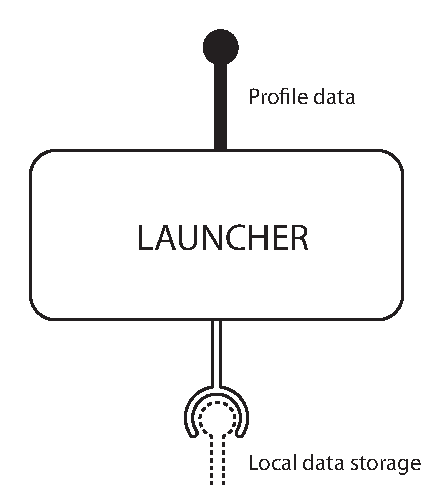
\includegraphics[width=0.5\textwidth]{gfx/external_launcher_architecture.pdf}
	\caption{The external architecture of the \giraf[] launcher.}
	\label{fig:external_architecture}
\end{figure}

%%%%%%%%%%%%%%%%%%%%%%%%%%%%%%%%%%%%%%%%%%%%%%%%%%%%%%%%%%%%%%%%%%%%%%%%%%%%%%%%%%%% COMMENT
\begin{comment}
Two external architectures are described in this section, namely those of the \giraf[] launcher, and the \guicomponents[] library.

\subsection{\giraf[] Launcher}
\label{sec:launcher_architecture}
The external architecture of the launcher can be seen in \autoref{fig:external_architecture}.
\begin{figure}[h]
	\centering
	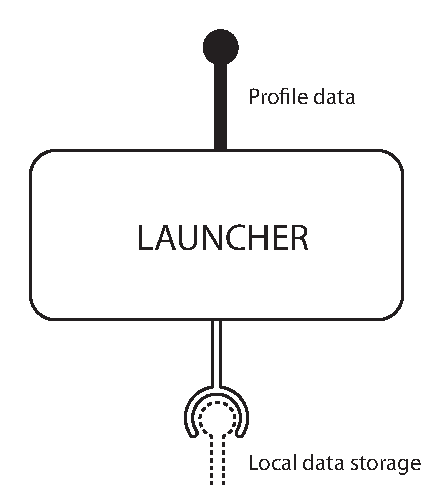
\includegraphics[width=0.5\textwidth]{gfx/external_launcher_architecture.pdf}
	\caption{The external architecture of the \giraf[] launcher.}
	\label{fig:external_architecture}
\end{figure}
The launcher provides two essential services: The ability for users to run, i.e. \textit{launch}, apps, and the provisioning of profile data to these apps. 
The launcher currently allows only \giraf[] apps to be used, but this is by design, as the launcher currently does not support addition and removal of apps. 
The profile data service allows a \guardian[] profile to select a child profile to use a given app with. 
Both the ID of the \guardian[] profile and the child profile is then provided to the app, in order to make it easy for a \guardian[] to switch between different children as needed, while maintaining specific app customizations for different profiles. \newline

The \giraf[] launcher has only one dependancy in the \giraf[] system, namely the Oasis database. 
The launcher is heavily integrated with Oasis, and as such requires the Oasis database to be installed on the device to function. 
Services utilized by the launcher include profile authentication, saving and loading of settings and app integration. 

\subsection{\guicomponents[]}
The \guicomponents[] architecture is designed to be flexible. 
The flexibility is important to keep the \guicomponents[] open and changeable by anyone involved in the development of \giraf[]. 
As such, the only architectural requirement for components that are added to \guicomponents[], is that they should be based on existing Android UI components. 
The philosophy behind this architecture, is that by using existing Android UI components, with a new layout and possible added functionality, the components are already well defined and fully supported in Android. 
The example shown in \autoref{fig:gui_comp_architecture} highlights a possible way of incorporating a component, assuming the need for a customized button: \textit{GButton}. 
\begin{figure}[h]
	\centering
	
\includegraphics[width=1\textwidth]{gfx/gui_components_architecture.pdf}
	\caption{\guicomponents[] Architecture Example}
	\label{fig:gui_comp_architecture}
\end{figure}
\end{comment}
\section{Internal Architecture}

Being able to launch an \girafapp[] as a specific guardian requires that the user interacts such that the launcher knows which guardian the user represents.

Authentication is chosen, as each modulated child and guardian contains private data. QR-codes are chosen as means of authentication, as they provide a level of security.

An alternative to QR-codes could be a \emph{username-password} method, where each user have their own username, with an private password. The system is designed to have the two modes: guardian- and child mode\todo{ref til backlog}. A username-password combination requires the user to remember their credentials, whereas some \autists[] have problems with it. \todo{quote drazenko - vent paa mail fra accept}

%\myquote{Some children with autism can have a hard time remembering a username and a password}
 - Drazenko Banjak, english translation. Native language quote can be seen in \autoref{FIXME}\todo{indsaet i appendix "Nogle børn med autisme kan have svært ved at skulle huske et brugernavn og en adgangskode."}

QR codes provides a physical way of storing the user credentials and allows for other users to take responsibility of the QR-code, such as a \guardian[] carrying a QR-code of a \autist[].

QR-codes can be scanned by a built-in camera on tablets and can be printed using standard paper and printer equipment. 

QR-codes are copyable, by e.g. a copymachine, and therefore must be kept away from untrusted users, if they should not be used by people for which they were not intended.

To sum up, QR-codes are chosen because of they improve usability, despite of their ability to be copied.\todo{Ulrik, er dette i orden?}


%%%%%%%%%%%%%%%%%%%%%%%%%%%%%%%%%%%%%%%%%%%%%% COMMENT
\begin{comment}
\begin{figure}[h]
	\centering
	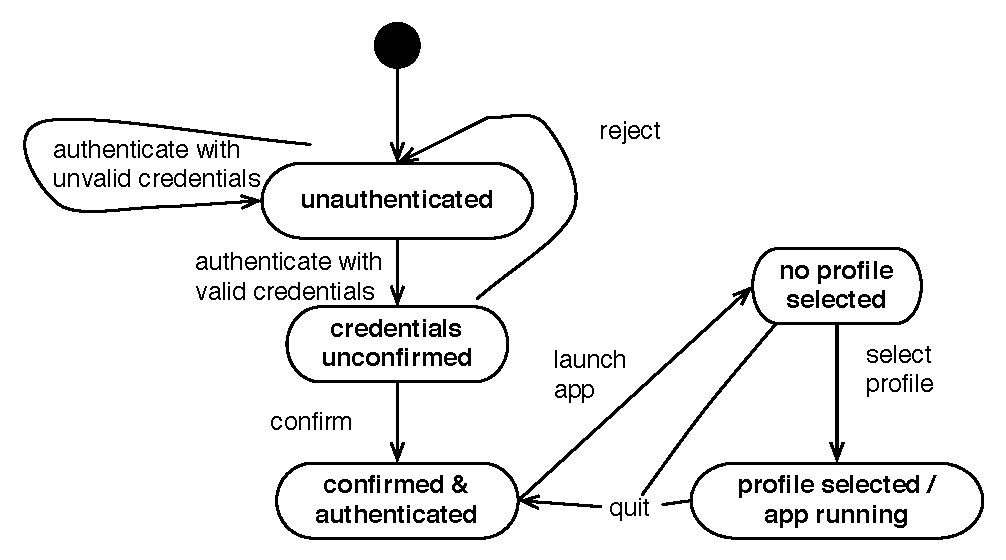
\includegraphics[width=1\textwidth]{gfx/flow-diagram2.pdf}
	\caption{Flow diagram}
	\label{fig:flow_diagram}
\end{figure}

\autoref{fig:flow_diagram} shows the state of the launcher. The first three states handles the distinction between users which are allowed to access the launchable applications, and those who are not. \todo{indsaet ref til der hvor vi fandt ud af at vi skulle have authentication}

Based on \autoref{fig:flow_diagram}, ..
\end{comment}





%\cleardoublepage
\cleardoublepage
% Table of Contents - List of Tables/Figures/Listings and Acronyms

\refstepcounter{dummy}

\pdfbookmark[1]{\contentsname}{tableofcontents} % Bookmark name visible in a PDF viewer

\setcounter{tocdepth}{2} % Depth of sections to include in the table of contents - currently up to subsections

\setcounter{secnumdepth}{3} % Depth of sections to number in the text itself - currently up to subsubsections

\manualmark
\markboth{\spacedlowsmallcaps{\contentsname}}{\spacedlowsmallcaps{\contentsname}}

\tableofcontents 

\automark[section]{chapter}
\renewcommand{\chaptermark}[1]{\markboth{\spacedlowsmallcaps{#1}}{\spacedlowsmallcaps{#1}}}
\renewcommand{\sectionmark}[1]{\markright{\thesection\enspace\spacedlowsmallcaps{#1}}}

\clearpage

\begingroup 
\let\clearpage\relax
\let\cleardoublepage\relax
\let\cleardoublepage\relax

%----------------------------------------------------------------------------------------
%	List of Figures
%----------------------------------------------------------------------------------------

\refstepcounter{dummy}
%\addcontentsline{toc}{chapter}{\listfigurename} % Uncomment if you would like the list of figures to appear in the table of contents
\pdfbookmark[1]{\listfigurename}{lof} % Bookmark name visible in a PDF viewer

\listoffigures

\vspace*{8ex}
\newpage

%----------------------------------------------------------------------------------------
%	List of Tables
%----------------------------------------------------------------------------------------

\refstepcounter{dummy}
%\addcontentsline{toc}{chapter}{\listtablename} % Uncomment if you would like the list of tables to appear in the table of contents
\pdfbookmark[1]{\listtablename}{lot} % Bookmark name visible in a PDF viewer

\listoftables
        
\vspace*{8ex}
\newpage
    
%----------------------------------------------------------------------------------------
%	List of Listings
%---------------------------------------------------------------------------------------- 

\refstepcounter{dummy}
%\addcontentsline{toc}{chapter}{\lstlistlistingname} % Uncomment if you would like the list of listings to appear in the table of contents
\pdfbookmark[1]{\lstlistlistingname}{lol} % Bookmark name visible in a PDF viewer

\lstlistoflistings 

\vspace*{8ex}
\newpage
       
%----------------------------------------------------------------------------------------
%	Acronyms
%----------------------------------------------------------------------------------------

\refstepcounter{dummy}
%\addcontentsline{toc}{chapter}{Acronyms} % Uncomment if you would like the acronyms to appear in the table of contents
\pdfbookmark[1]{Acronyms}{acronyms} % Bookmark name visible in a PDF viewer

\markboth{\spacedlowsmallcaps{Acronyms}}{\spacedlowsmallcaps{Acronyms}}

\chapter*{Acronyms}

\begin{acronym}[UML]
%\acro{DRY}{Don't Repeat Yourself}
\end{acronym}  
                   
\endgroup

\cleardoublepage % Contents, list of figures/tables/listings and acronyms

\pagenumbering{arabic} % Arabic page numbering for thesis content (1, 2, 3, etc)
%\setcounter{page}{90} % Uncomment to manually start the page counter at an arbitrary value (for example if you wish to count the pre-content pages in the page count)

\cleardoublepage % Avoids problems with pdfbookmark

%----------------------------------------------------------------------------------------
%	INTRODUCTION
%----------------------------------------------------------------------------------------



\section{External Architecture}

\autoref{fig:external_architecture} illustrates the \giraf[] launcher component. The component provides one service and have one dependency. The services it provides is based on demands from the surrounding components of the \giraf[] platform, which can be seen in \autoref{cmn:fig:architecture}. The illustrated service provides a way for launched \girafapp[]s to determine which guardian launched the application in question, and with which child profile. The illustrated dependency represents the need for being able to read and update profile data. The service which fulfill this dependency is provided by Oasis. 

As seen on \autoref{cmn:fig:architecture}, Oasis is available for the launcher to use. This database stores the modulated data, including the guardian and child profiles.


\begin{figure}[h]
	\centering
	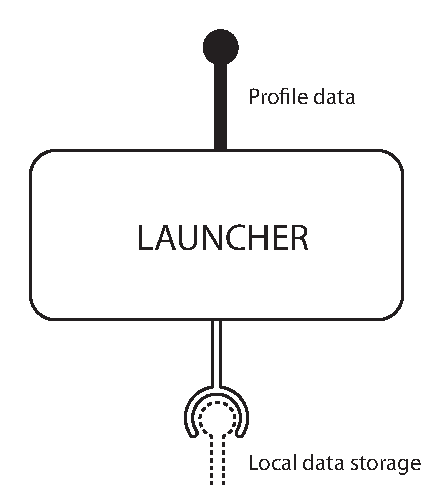
\includegraphics[width=0.5\textwidth]{gfx/external_launcher_architecture.pdf}
	\caption{The external architecture of the \giraf[] launcher.}
	\label{fig:external_architecture}
\end{figure}

%%%%%%%%%%%%%%%%%%%%%%%%%%%%%%%%%%%%%%%%%%%%%%%%%%%%%%%%%%%%%%%%%%%%%%%%%%%%%%%%%%%% COMMENT
\begin{comment}
Two external architectures are described in this section, namely those of the \giraf[] launcher, and the \guicomponents[] library.

\subsection{\giraf[] Launcher}
\label{sec:launcher_architecture}
The external architecture of the launcher can be seen in \autoref{fig:external_architecture}.
\begin{figure}[h]
	\centering
	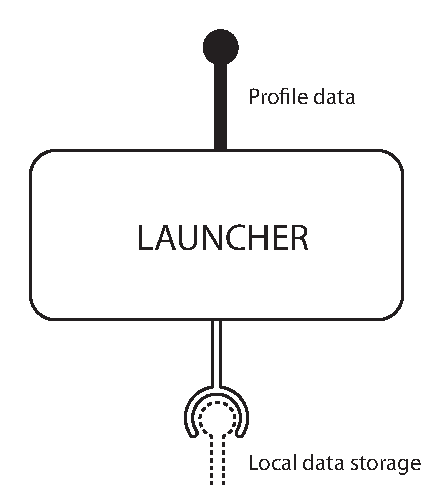
\includegraphics[width=0.5\textwidth]{gfx/external_launcher_architecture.pdf}
	\caption{The external architecture of the \giraf[] launcher.}
	\label{fig:external_architecture}
\end{figure}
The launcher provides two essential services: The ability for users to run, i.e. \textit{launch}, apps, and the provisioning of profile data to these apps. 
The launcher currently allows only \giraf[] apps to be used, but this is by design, as the launcher currently does not support addition and removal of apps. 
The profile data service allows a \guardian[] profile to select a child profile to use a given app with. 
Both the ID of the \guardian[] profile and the child profile is then provided to the app, in order to make it easy for a \guardian[] to switch between different children as needed, while maintaining specific app customizations for different profiles. \newline

The \giraf[] launcher has only one dependancy in the \giraf[] system, namely the Oasis database. 
The launcher is heavily integrated with Oasis, and as such requires the Oasis database to be installed on the device to function. 
Services utilized by the launcher include profile authentication, saving and loading of settings and app integration. 

\subsection{\guicomponents[]}
The \guicomponents[] architecture is designed to be flexible. 
The flexibility is important to keep the \guicomponents[] open and changeable by anyone involved in the development of \giraf[]. 
As such, the only architectural requirement for components that are added to \guicomponents[], is that they should be based on existing Android UI components. 
The philosophy behind this architecture, is that by using existing Android UI components, with a new layout and possible added functionality, the components are already well defined and fully supported in Android. 
The example shown in \autoref{fig:gui_comp_architecture} highlights a possible way of incorporating a component, assuming the need for a customized button: \textit{GButton}. 
\begin{figure}[h]
	\centering
	
\includegraphics[width=1\textwidth]{gfx/gui_components_architecture.pdf}
	\caption{\guicomponents[] Architecture Example}
	\label{fig:gui_comp_architecture}
\end{figure}
\end{comment}
\section{Internal Architecture}

Being able to launch an \girafapp[] as a specific guardian requires that the user interacts such that the launcher knows which guardian the user represents.

Authentication is chosen, as each modulated child and guardian contains private data. QR-codes are chosen as means of authentication, as they provide a level of security.

An alternative to QR-codes could be a \emph{username-password} method, where each user have their own username, with an private password. The system is designed to have the two modes: guardian- and child mode\todo{ref til backlog}. A username-password combination requires the user to remember their credentials, whereas some \autists[] have problems with it. \todo{quote drazenko - vent paa mail fra accept}

%\myquote{Some children with autism can have a hard time remembering a username and a password}
 - Drazenko Banjak, english translation. Native language quote can be seen in \autoref{FIXME}\todo{indsaet i appendix "Nogle børn med autisme kan have svært ved at skulle huske et brugernavn og en adgangskode."}

QR codes provides a physical way of storing the user credentials and allows for other users to take responsibility of the QR-code, such as a \guardian[] carrying a QR-code of a \autist[].

QR-codes can be scanned by a built-in camera on tablets and can be printed using standard paper and printer equipment. 

QR-codes are copyable, by e.g. a copymachine, and therefore must be kept away from untrusted users, if they should not be used by people for which they were not intended.

To sum up, QR-codes are chosen because of they improve usability, despite of their ability to be copied.\todo{Ulrik, er dette i orden?}


%%%%%%%%%%%%%%%%%%%%%%%%%%%%%%%%%%%%%%%%%%%%%% COMMENT
\begin{comment}
\begin{figure}[h]
	\centering
	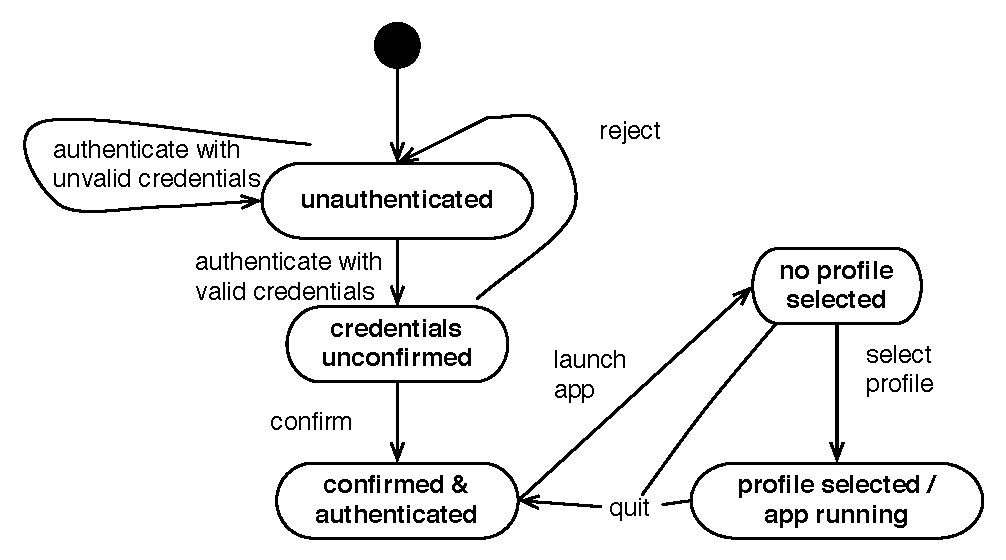
\includegraphics[width=1\textwidth]{gfx/flow-diagram2.pdf}
	\caption{Flow diagram}
	\label{fig:flow_diagram}
\end{figure}

\autoref{fig:flow_diagram} shows the state of the launcher. The first three states handles the distinction between users which are allowed to access the launchable applications, and those who are not. \todo{indsaet ref til der hvor vi fandt ud af at vi skulle have authentication}

Based on \autoref{fig:flow_diagram}, ..
\end{comment}



%----------------------------------------------------------------------------------------
%	POST-CONTENT
%----------------------------------------------------------------------------------------

\cleardoublepage% Bibliography

\label{app:bibliography} % Reference the bibliography elsewhere with \autoref{app:bibliography}

\manualmark
\markboth{\spacedlowsmallcaps{\bibname}}{\spacedlowsmallcaps{\bibname}} 
\refstepcounter{dummy}

\addtocontents{toc}{\protect\vspace{\beforebibskip}} % Place the bibliography slightly below the rest of the document content in the table of contents
\addcontentsline{toc}{chapter}{\tocEntry{\bibname}}

\bibliographystyle{plainnat}

\bibliography{Bibliography} % Bibliography

%----------------------------------------------------------------------------------------

\end{document}
